\documentclass[margin=5mm]{standalone}

\usepackage{tikz}
\usetikzlibrary{calc}
\begin{document}

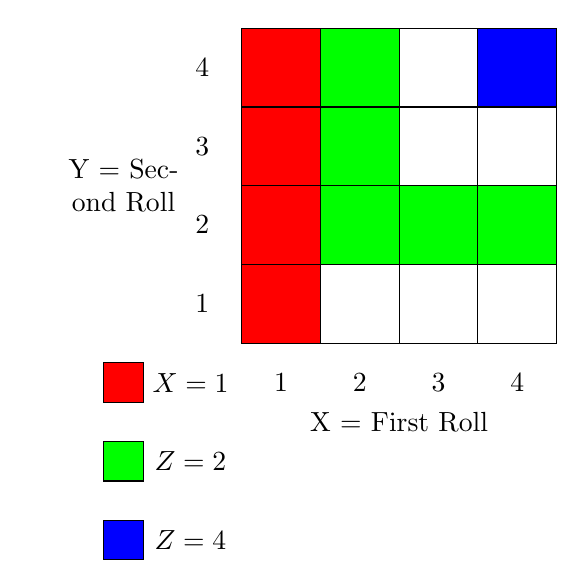
\begin{tikzpicture}
  \draw (-2,-2) grid (2,2);
  \foreach \x/\xtext in {-1.5/1, -0.5/2, 0.5/3, 1.5/4} {
    \draw (\x, -2.5) node {\xtext};
    \draw (-2.5, \x) node {\xtext};
  }
  \draw (0, -3) node {X = First Roll};
  \draw (-3.5, 0) node[align=center, text width=2.2cm] {Y = Second Roll};

  \foreach \x/\xtext in {-1.5/1, -0.5/2, 0.5/3, 1.5/4} {
    \draw [fill=red] ($(-2, \x-0.5)$) rectangle ($(-1, \x+0.5)$);
  }
  \draw [fill=red] (-3.75, -2.75) rectangle (-3.25, -2.25);
  \draw (-2.65, -2.5) node {$X=1$};

  \foreach \x/\xtext in {-0.5/2, 0.5/3, 1.5/4} {
    \draw [fill=green] ($(-1, \x-0.5)$) rectangle ($(0, \x+0.5)$);
  }

  \foreach \x/\xtext in {-0.5/2, 0.5/3, 1.5/4} {
    \draw [fill=green] ($(\x-0.5, -1)$) rectangle ($(\x+0.5, 0)$);
  }
  \draw [fill=green] (-3.75, -3.75) rectangle (-3.25, -3.25);
  \draw (-2.65, -3.5) node {$Z=2$};

  \draw [fill=blue] (1,1) rectangle (2,2);
  \draw [fill=blue] (-3.75, -4.75) rectangle (-3.25, -4.25);
  \draw (-2.65, -4.5) node {$Z=4$};
\end{tikzpicture}
\end{document}
